\section{Applied $\pi$-Calculus}
%Short - examples of the applied $\pi$-calculus 
%\begin{itemize}
%  \item General about Applied Pi Calculus, and how it differs from pi calculus (terms; in particular for security protocols)
%  \item Examples of applied pi calculus (handshake protocol?)
%  \item ProVerif - automatic symbolic protocol verifier
%\end{itemize}

The applied pi-calculus (ref. Abadi and Fournet, 2001) is based upon the language pi-calculus, but offers a more convenient use for modelling security protocols to be specified, by allowing for a more wide variety of complex primitives. It is used for describing and analysing security protocols, as it provides a more intuitive process syntax for detailing the actions of the participants in a protocol \autocite{AplliedPiCalsulus2010}. This is done by introducing a rich term algebra, for modelling the cryptographic operations used in security protocols, where function symbols represent cryptographic protocols. 

Tools such as ProVerif \autocite{ProVerif}, uses a syntax closely related to the applied pi-calculus, and offers a way of automated reasoning about the security properties found in cryptographic protocols. \\
%- The properties of these primitives are modelled by equations \\ 

%"The applied pi calculus (...) is a language for describing concurrent processes and their interactions". \\
\subsection{Terms}
As mentioned, the applied pi-calculus uses Terms (in contrast to just names in the pi-calculus) to model messages that are exchanged during a protocol. Terms are built over a signature, names and variables\autocite{AplliedPiCalsulus2010}: \\
\begin{center}
	\begin{tabular} { l l }
 		L, M, N, T, U, V ::= & terms \\ 
 		a, b, c,...,k,...,m, n,..,s & names \\  
 		x, y, z & variables \\
 		g(M$_{1}$,..,M$_{l}$) & function application
		%\caption{Fig. 1.1}
		%\label{tbl:excel-table}
	\end{tabular}
\end{center}


\subsection{Examples}
Having established an understanding of how the the applied pi-calculus differentiate from the pi-calculus, we can now look at how some of the known protocols can be described.\\
First of, we look at the simple Handshake protocol used for setting the parameters for communication between two devices, such as the old dial-up modem or when connecting to a USB.  \\
Handshake protocol with applied pi-calculus as illustred by \citeauthor{AplliedPiCalsulus2010}:
\begin{center}
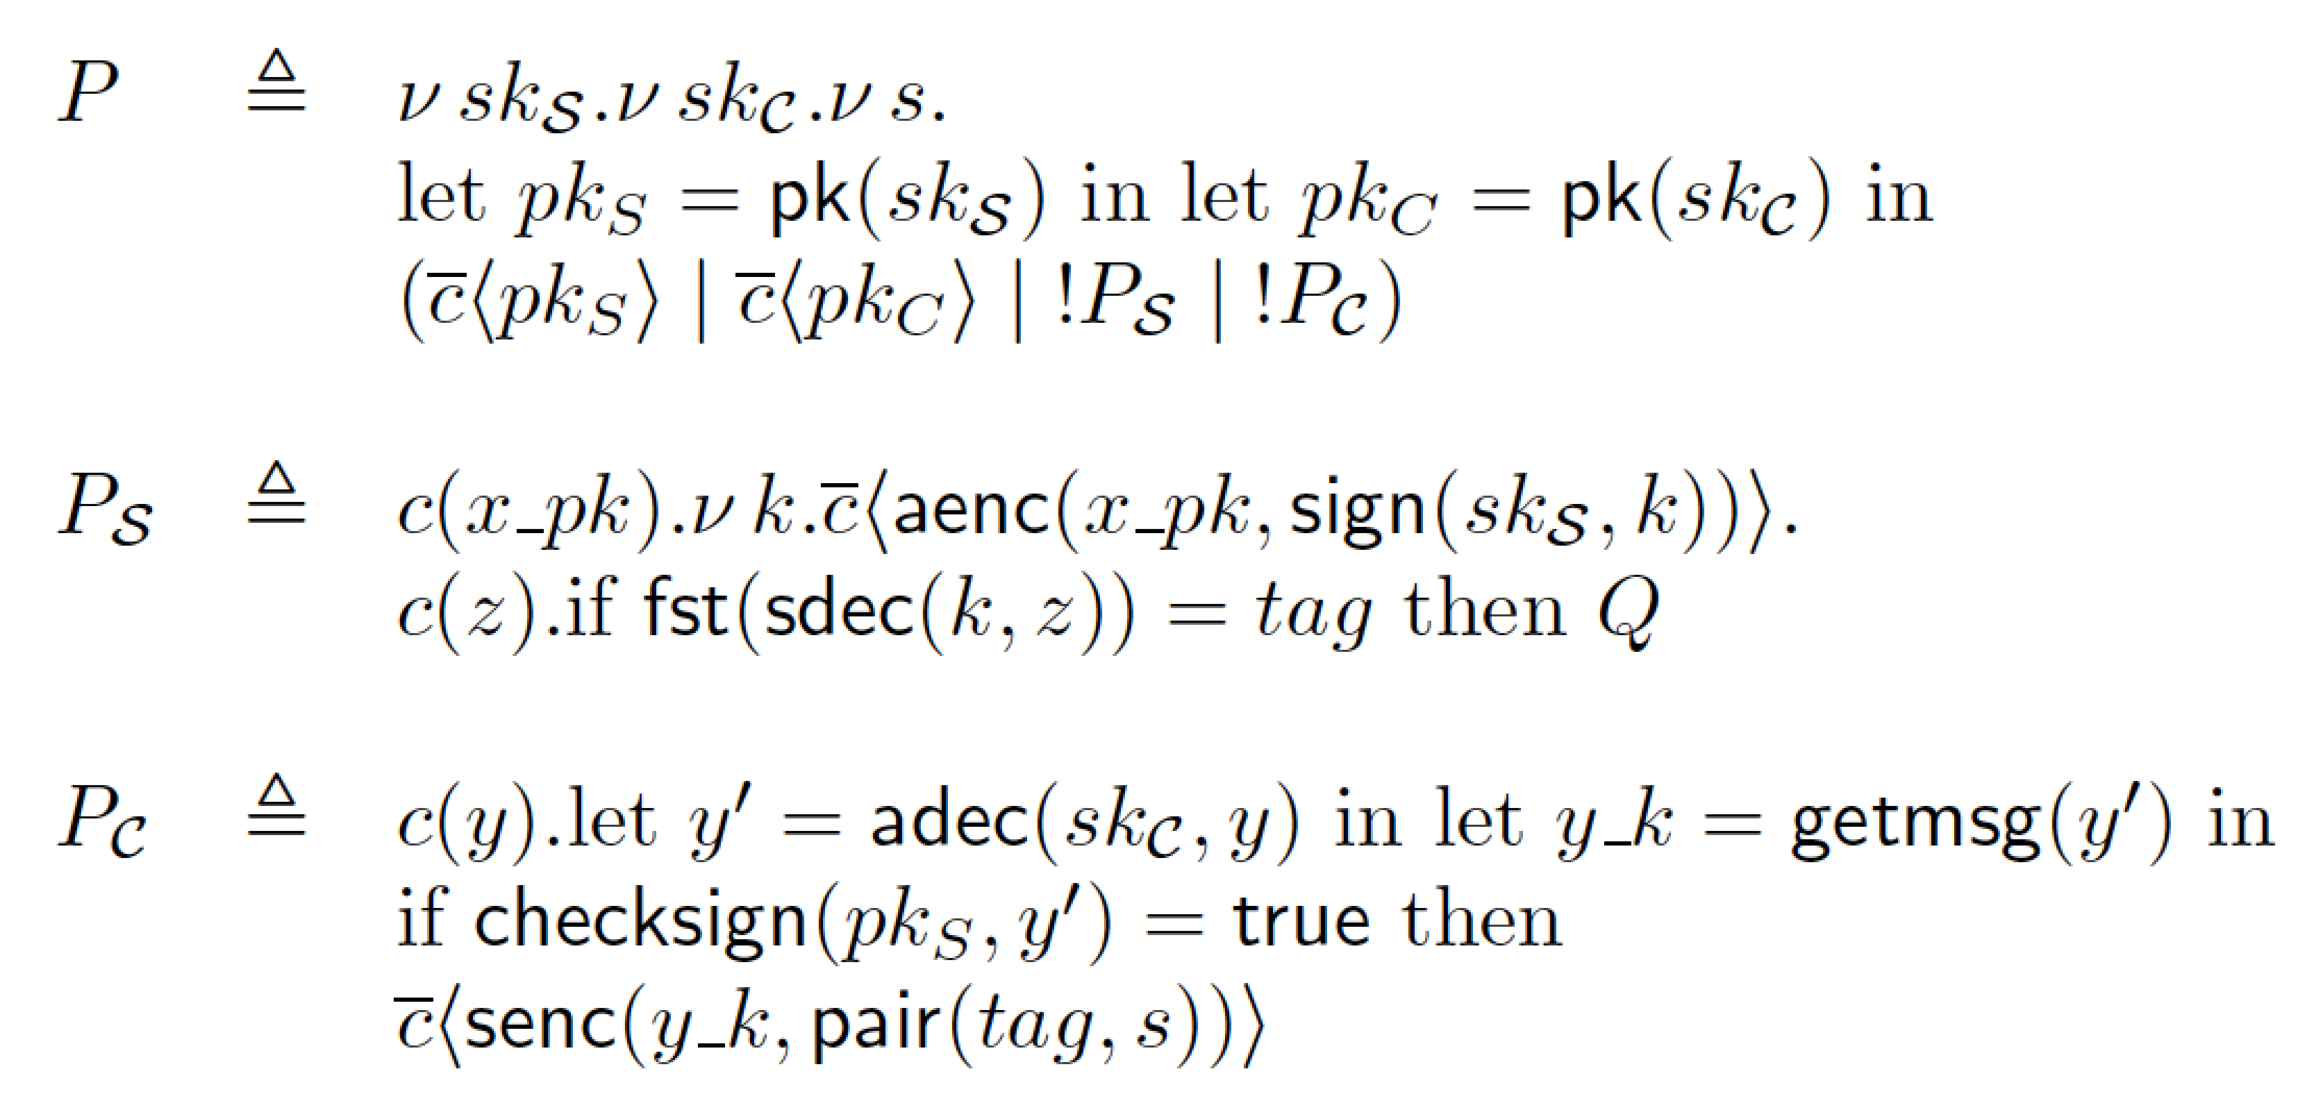
\includegraphics[width=0.7\textwidth, angle=0]{Handshake.pdf}
\end{center}
Needham-Schroeder Public key protocol with applied pi-calculus by \citeauthor{DBLP:journals/ftpl/CortierK14,}:
\begin{center}
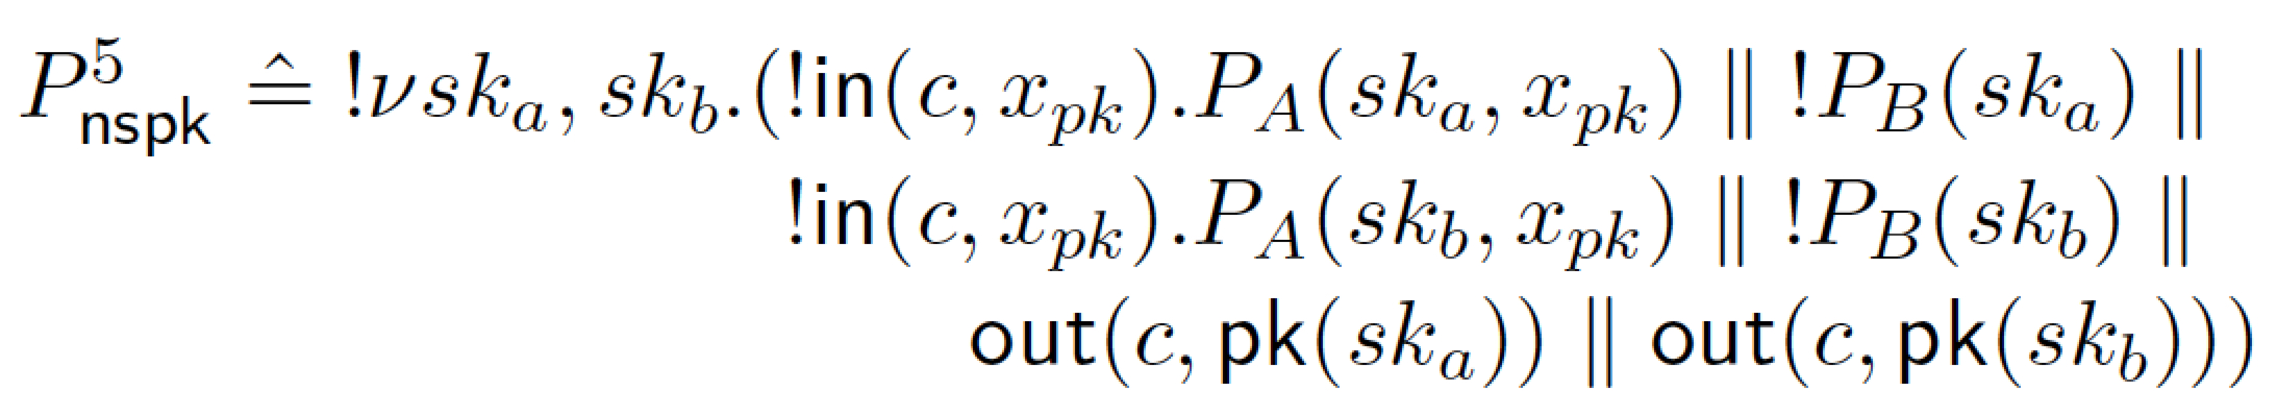
\includegraphics[width=0.7\textwidth, angle=0]{Needham_Schroeder.pdf}
\end{center}
TODO: Do description and explanation of both 
